% !TEX program = xelatex
% AY2012 材料力学 解答例（同志社 生命医科学 医工学コース 院試）
% 問題・図は 01_exams/2012/tex を土台に、参考/ の粒度で解答を付した。
\documentclass[11pt,a4paper]{article}
\usepackage{../../00_common/preamble}
\usetikzlibrary{positioning,arrows.meta,calc,patterns,decorations.pathmorphing}

\title{材料力学 AY2012 解答例（専門応用科目I）}
\author{}
\date{}

\begin{document}
\maketitle

\noindent\textbf{符号規約}：反力・たわみは上向きを正，集中荷重 $P$ は下向き．
せん断力 $Q$ は断面左側に働く上向き外力の和，曲げモーメント $M$ は下に凸（さがり）を正とし，
たわみの基礎式は $EI\,\dfrac{d^2v}{dx^2}=M(x)$ を用いる．

%====================================================================
\section*{〔I〕}

図に示す単純支持・突き出しはりの右端 $C$ 点に集中荷重 $P$ が負荷される問題に答えよ.
ヤング率（縦弾性係数）を $E$, はりの断面二次モーメントを $I$ とせよ.

\begin{center}
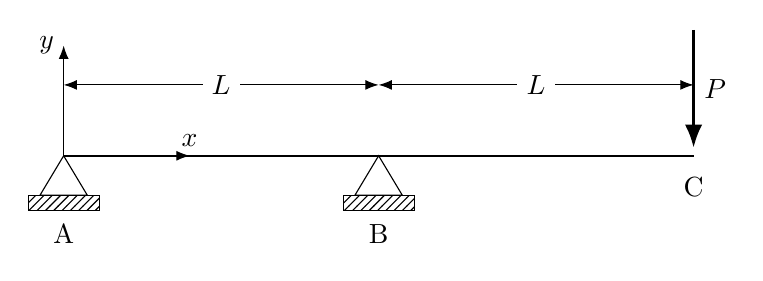
\begin{tikzpicture}[>=Latex]
  \draw[thick] (0,0) -- (8,0);
  \draw[->] (0,0) -- (0,1.4) node[left]{$y$};
  \draw[->] (0,0) -- (1.6,0) node[above]{$x$};
  \draw (0,0) -- (-0.3,-0.5) -- (0.3,-0.5) -- cycle;
  \draw[pattern=north east lines] (-0.45,-0.7) rectangle (0.45,-0.5);
  \node at (0,-1.0) {A};
  \draw (4,0) -- (3.7,-0.5) -- (4.3,-0.5) -- cycle;
  \draw[pattern=north east lines] (3.55,-0.7) rectangle (4.45,-0.5);
  \node at (4,-1.0) {B};
  \node at (8,-0.4) {C};
  \draw[->,very thick] (8,1.6) -- (8,0.1) node[midway,right]{$P$};
  \draw[<->] (0,0.9) -- (4,0.9) node[midway,fill=white]{$L$};
  \draw[<->] (4,0.9) -- (8,0.9) node[midway,fill=white]{$L$};
\end{tikzpicture}
\end{center}

\begin{enumerate}[label=(\arabic*)]
  \item 支持点 A, B に生じる支持力を図示し, つり合い式によりそれらを求めよ.
  \item せん断力 $Q(x)$ と曲げモーメント $M(x)$ を求め, SFD と BMD を示せ.
  \item たわみ $v(x)$ に関するはりの基礎式を示し, たわみ角とたわみ曲線を求め, C 点におけるたわみを求めよ.
  \item C 点におけるたわみをカスチリアーノの定理（エネルギー法）を用いて求めよ.
\end{enumerate}

\subsection*{解答}

\noindent\textbf{(1)}\quad 支点 A の反力を $R_A$，支点 B の反力を $R_B$（ともに上向き正）とおく．
鉛直方向の力のつり合いと，点 A まわりのモーメントのつり合いより
\[
  R_A + R_B - P = 0, \qquad R_B\cdot L - P\cdot 2L = 0.
\]
第2式より $R_B = 2P$，これを第1式へ代入して $R_A = P - R_B = -P$．
\[
  \ans{\,R_A = -P\ (\text{下向き}),\qquad R_B = 2P\ (\text{上向き})\,}
\]
検算：$R_A + R_B = -P + 2P = P$（$=$ 外力 $P$）✓．

\medskip
\noindent\textbf{(2)}\quad 断面左側のつり合いを区間ごとにとる．

\noindent(I)\ $0\le x<L$（区間 AB）：
\[
  Q(x) = R_A = -P, \qquad M(x) = R_A x = -Px.
\]
(II)\ $L\le x\le 2L$（区間 BC）：
\[
  Q(x) = R_A + R_B = P, \qquad M(x) = R_A x + R_B(x-L) = Px - 2PL.
\]
端点・接続点の値：$M(0)=0$，$M(L)=-PL$，$M(2L)=0$（自由端で 0）．
\[
  \ans{\,Q(x)=\begin{cases}-P & (0\le x<L)\\ P & (L\le x\le 2L)\end{cases}
  \qquad
  M(x)=\begin{cases}-Px & (0\le x<L)\\ Px-2PL & (L\le x\le 2L)\end{cases}\,}
\]

\begin{center}
\begin{tikzpicture}[>=Latex,scale=1.0]
  \def\L{2.6}
  \begin{scope}
    \draw[->] (-0.3,0) -- (2*\L+0.6,0) node[right]{$x$};
    \draw[->] (0,-1.1) -- (0,1.1) node[above]{SFD};
    \draw[line width=1pt,blue] (0,-0.7) -- (\L,-0.7) -- (\L,0.7) -- (2*\L,0.7);
    \node[left] at (0,-0.7) {$-P$}; \node[left] at (0,0.7) {$P$};
    \node[below] at (\L,0) {$L$}; \node[below] at (2*\L,0) {$2L$};
  \end{scope}
  \begin{scope}[xshift=8.5cm]
    \draw[->] (-0.3,0) -- (2*\L+0.6,0) node[right]{$x$};
    \draw[->] (0,-1.2) -- (0,0.8) node[above]{BMD};
    \draw[line width=1pt,red] (0,0) -- (\L,-1.0) -- (2*\L,0);
    \node[below left] at (\L,-1.0) {$-PL$};
    \node[above] at (0,0) {$A$}; \node[below] at (\L,0) {$B$}; \node[above] at (2*\L,0) {$C$};
  \end{scope}
\end{tikzpicture}
\end{center}

\medskip
\noindent\textbf{(3)}\quad たわみの基礎式 $EI\,v''=M(x)$ を各区間で2回積分する（$\times EI$ で表す）．
\[
  EI\,v_1' = -\frac{P}{2}x^2 + C_1,\quad EI\,v_1 = -\frac{P}{6}x^3 + C_1 x + C_2 \qquad(0\le x<L),
\]
\[
  EI\,v_2' = \frac{P}{2}x^2 - 2PL\,x + C_3,\quad EI\,v_2 = \frac{P}{6}x^3 - PL\,x^2 + C_3 x + C_4 \qquad(L\le x\le 2L).
\]
境界条件 $v_1(0)=0,\ v_1(L)=0$ と接続条件 $v_1(L)=v_2(L),\ v_1'(L)=v_2'(L)$ より
\[
  C_2=0,\quad C_1=\frac{PL^2}{6},\quad C_3=\frac{7PL^2}{6},\quad C_4=-\frac{PL^3}{3}.
\]
よってたわみ角・たわみ曲線は
\[
  \ans{\;EI\,v_1 = -\frac{P}{6}x^3 + \frac{PL^2}{6}x,\qquad
        EI\,v_2 = \frac{P}{6}x^3 - PL\,x^2 + \frac{7PL^2}{6}x - \frac{PL^3}{3}\;}
\]
C 点（$x=2L$）のたわみは
\[
  EI\,v_2(2L) = \frac{P}{6}(2L)^3 - PL(2L)^2 + \frac{7PL^2}{6}(2L) - \frac{PL^3}{3} = -\frac{2PL^3}{3}.
\]
\[
  \ans{\;v_C = -\frac{2PL^3}{3EI}\quad(\text{下向きに } \tfrac{2PL^3}{3EI})\;}
\]

\begin{center}
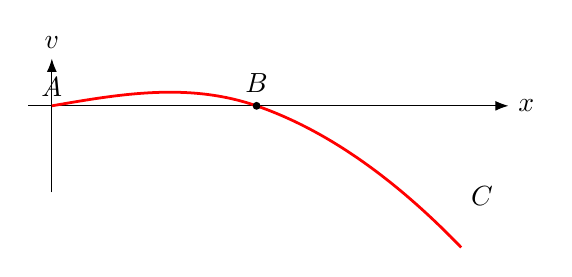
\begin{tikzpicture}[>=Latex,scale=1.0]
  \def\L{2.6}
  \draw[->] (-0.3,0) -- (2*\L+0.6,0) node[right]{$x$};
  \draw[->] (0,-1.1) -- (0,0.6) node[above]{$v$};
  \draw[line width=1pt,red,smooth,samples=60,domain=0:1] plot (\L*\x,{0.5*(-(\x*\x*\x)+(\x))*0.9});
  \draw[line width=1pt,red,smooth,samples=60,domain=1:2] plot (\L*\x,{-0.9*(\x-1)*(\x)});
  \node[above] at (0,0) {$A$}; \fill (\L,0) circle (0.05); \node[above] at (\L,0.05) {$B$};
  \node[below right] at (2*\L,-0.9) {$C$};
\end{tikzpicture}
\end{center}
検算：$v_1(0)=0,\ v_1(L)=0$（両支点で 0），接続点 $v_1(L)=v_2(L)$ が一致 ✓．

\medskip
\noindent\textbf{(4)}\quad カスチリアーノの定理 $\displaystyle \delta_C=\frac{\partial U}{\partial P}=\int \frac{M}{EI}\frac{\partial M}{\partial P}\,dx$ を用いる．
区間 I では $M_1=-Px,\ \dfrac{\partial M_1}{\partial P}=-x$，区間 II では $M_2=P(x-2L),\ \dfrac{\partial M_2}{\partial P}=x-2L$ であるから
\[
  \delta_C = \frac{1}{EI}\left[\int_0^L (-Px)(-x)\,dx + \int_L^{2L} P(x-2L)(x-2L)\,dx\right]
  = \frac{1}{EI}\left(\frac{PL^3}{3}+\frac{PL^3}{3}\right).
\]
\[
  \ans{\;\delta_C = \frac{2PL^3}{3EI}\quad(\text{荷重 }P\text{ の向き，すなわち下向き})\;}
\]
検算：(3) のたわみ曲線から得た $|v_C|=\dfrac{2PL^3}{3EI}$ と一致する ✓．

%====================================================================
\clearpage
\section*{〔II〕}

図に示す上端を固定された板厚一定の台形板（上端と下端の幅 $b_2$, $b_1$）の
引張り変形に関する問いに答えよ. 自重は無視せよ. 座標 $x$ の原点を棒の下端 B 点にとるものとする.

\begin{center}
\begin{tikzpicture}[>=Latex]
  \def\Hh{5}\def\Wt{2.4}\def\Wb{0.5}
  \draw[thick] (-\Wt,\Hh) -- (\Wt,\Hh) -- (\Wb,0) -- (-\Wb,0) -- cycle;
  \draw[pattern=north east lines] (-\Wt-0.2,\Hh) rectangle (\Wt+0.2,\Hh+0.25);
  \draw[<->] (-\Wt,\Hh+0.55) -- (\Wt,\Hh+0.55) node[midway,fill=white]{幅 $b_2$};
  \draw[<->] (-\Wb,-0.5) -- (\Wb,-0.5) node[midway,fill=white,font=\scriptsize]{幅 $b_1$};
  \node at (0,\Hh*0.62) {板厚 $t$};
  \draw[<->] (-1.25,1.8) -- (1.25,1.8) node[midway,fill=white,font=\scriptsize]{幅 $b(x)$};
  \draw[<->] (-\Wt-0.9,0) -- (-\Wt-0.9,\Hh) node[midway,fill=white]{$L$};
  \draw[->] (\Wt+0.6,0) -- (\Wt+0.6,2.2) node[above]{$x$};
  \node at (\Wt+0.35,\Hh) {A}; \node at (-0.7,-0.15) {B};
  \draw[->,very thick] (0,-0.55) -- (0,-1.8) node[midway,right]{$P$};
\end{tikzpicture}
\end{center}

\begin{enumerate}[label=(\arabic*)]
  \item 座標 $x$ における断面積 $A(x)$ を求めよ.
  \item 荷重 $P$ により座標 $x$ に生じる内力 $N(x)$ および応力 $\sigma(x)$ を求めよ.
  \item 棒全体の変位（伸び）$\lambda$ を求めよ.
\end{enumerate}

\subsection*{解答}

\noindent\textbf{(1)}\quad 下端 B（$x=0$）で幅 $b_1$，上端 A（$x=L$）で幅 $b_2$ であり，幅は $x$ について線形に変化する．
よって座標 $x$ での幅は
\[
  b(x) = b_1 + \frac{b_2-b_1}{L}\,x.
\]
板厚 $t$ は一定であるから断面積は
\[
  \ans{\;A(x) = t\,b(x) = t\left(b_1 + \frac{b_2-b_1}{L}\,x\right)\;}
\]
検算：$A(0)=t\,b_1$，$A(L)=t\,b_2$（上下端の幅に一致）✓．

\medskip
\noindent\textbf{(2)}\quad 自重を無視するので，任意断面で軸力は荷重 $P$ に等しい（引張り）．したがって
\[
  \ans{\;N(x) = P,\qquad \sigma(x) = \frac{N(x)}{A(x)} = \frac{P}{t\left(b_1 + \dfrac{b_2-b_1}{L}x\right)}\;}
\]

\medskip
\noindent\textbf{(3)}\quad 微小要素 $dx$ の伸びは $d\lambda = \dfrac{\sigma(x)}{E}\,dx = \dfrac{P}{E\,A(x)}\,dx$．全長にわたり積分して
\[
  \lambda = \int_0^L \frac{P}{E\,t\!\left(b_1 + \frac{b_2-b_1}{L}x\right)}\,dx
         = \frac{P}{Et}\cdot\frac{L}{b_2-b_1}\Big[\ln\!\big(b_1 + \tfrac{b_2-b_1}{L}x\big)\Big]_0^L .
\]
\[
  \ans{\;\lambda = \frac{PL}{E\,t\,(b_2-b_1)}\,\ln\!\frac{b_2}{b_1}\;}
\]
検算：一様断面の極限 $b_2\to b_1$ では，$\dfrac{\ln(b_2/b_1)}{b_2-b_1}\to \dfrac{1}{b_1}$ より
$\lambda\to \dfrac{PL}{E\,t\,b_1}=\dfrac{PL}{EA}$ となり，一様棒の伸びの公式に一致する ✓．

\end{document}
